% SC3020 --- Chapter 3: Classification (0->100 ground-up)
\chapter{Classification}
\label{ch:classification}

\begin{quote}
\emph{``Classification is prediction with a finite answer.''} Will this email be spam? Which disease does this X-ray show? We formalise classifiers that map inputs to discrete labels.
\end{quote}

\noindent\fbox{\parbox{\dimexpr\linewidth-2\fboxsep-2\fboxrule}{%
\textbf{From zero: no classifier assumed.} We start from a doctor's yes/no rule, formalise the learning problem, then build three canonical classifiers from intuition to formula: decision trees, Naive Bayes, and $k$-nearest neighbours. Pictures precede proofs.}}
\vspace{0.4em}

\section*{Learning Outcomes}
After this chapter you will be able to:
\begin{enumerate}[label=(L\arabic*)]
    \item formalise classification (input space, label space, hypothesis, loss);
    \item build and prune a decision tree using entropy and information gain;
    \item derive and apply Naive Bayes (Bayes rule $+$ conditional independence);
    \item apply $k$NN with distance metrics and discuss the curse of dimensionality;
    \item compute confusion-matrix metrics (accuracy, precision, recall, $F_1$).
\end{enumerate}

% ============================================================
\section{The Classification Problem}
\label{sec:class-problem}
\paragraph{Intuition.} Each patient is a point in feature space (fever, cough, age) coloured by a hidden label (flu or cold). Learning draws coloured regions so future points can be coloured by region. Errors happen where regions overlap.

\paragraph{Formal setup.} Input $\mathbf{x}\in\mathcal{X}\subseteq\mathbb{R}^d$, label $y\in\mathcal{Y}=\{1,\dots,C\}$. Training data $\mathcal{D}=\{(\mathbf{x}_i,y_i)\}_{i=1}^n\sim P(\mathbf{x},y)$. A hypothesis $h:\mathcal{X}\to\mathcal{Y}$ incurs loss $\ell(h(\mathbf{x}),y)$, often 0-1 loss. Empirical risk $\hat{R}(h)=\frac1n\sum_i\ell(h(\mathbf{x}_i),y_i)$ approximates true risk $R(h)=\mathbb{E}_{P}[\ell]$. A \emph{decision boundary} is $\{\mathbf{x}: h(\mathbf{x})\text{ changes}\}$. Good models balance fit and generalisation (bias-variance, Ch.~4).

% ============================================================
\section{Decision Trees}
\label{sec:trees}
\paragraph{Intuition.} A tree asks a sequence of yes/no questions (is fever $>$ 38? is age $<$ 10?) that partitions space into axis-aligned rectangles, each voting its majority label. Trees are interpretable but greedy and prone to overfitting.

\paragraph{Formal criterion.} At node $S$ with class proportions $p_c$, impurity:
\begin{align}
\text{Entropy } H(S) &= -\sum_{c} p_c\log_2 p_c, \qquad
\text{Gini } G(S)=1-\sum_c p_c^2.
\end{align}
For split $S\to\{S_v\}$ on attribute $A$,
\begin{equation}
\text{Gain}(S,A)= H(S)-\sum_v \frac{|S_v|}{|S|}\,H(S_v),\qquad
\text{GainRatio}= \frac{\text{Gain}}{\text{SplitInfo}}.
\end{equation}
The learner greedily picks $\arg\max_A \text{Gain}$ (ID3/C4.5) or Gini reduction (CART), recurses, and stops when pure, no attributes remain, or a pruning criterion fires. \emph{Pruning}: pre-pruning (max depth, min samples) or post-pruning (cost-complexity: minimise $R_\alpha(T)=R(T)+\alpha|T|$).

\begin{figure}[h]\centering
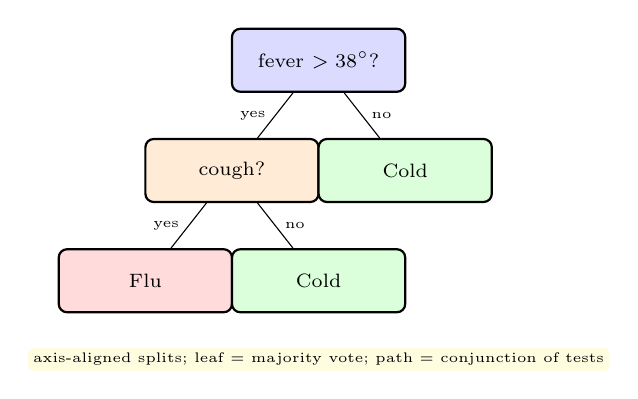
\begin{tikzpicture}[every node/.style={font=\scriptsize}, level distance=14mm, sibling distance=22mm,
  box/.style={draw, thick, rounded corners=3pt, align=center, minimum width=2.2cm, minimum height=0.8cm}]
\node[box, fill=blue!14] {fever $>38^\circ$?}
  child { node[box, fill=orange!16] {cough?}
    child { node[box, fill=red!14] {Flu} edge from parent node[left, font=\tiny] {yes} }
    child { node[box, fill=green!14] {Cold} edge from parent node[right, font=\tiny] {no} }
    edge from parent node[left, font=\tiny] {yes} }
  child { node[box, fill=green!14] {Cold} edge from parent node[right, font=\tiny] {no} };
\node[font=\tiny, fill=yellow!12, rounded corners=2pt, inner sep=2pt] at (0,-3.8) {axis-aligned splits; leaf = majority vote; path = conjunction of tests};
\end{tikzpicture}
\caption{A toy decision tree for diagnosis. Each internal node is a test; traversal from root to leaf applies the conjunction along the path.}
\label{fig:decision-tree}
\end{figure}

\begin{figure}[h]\centering
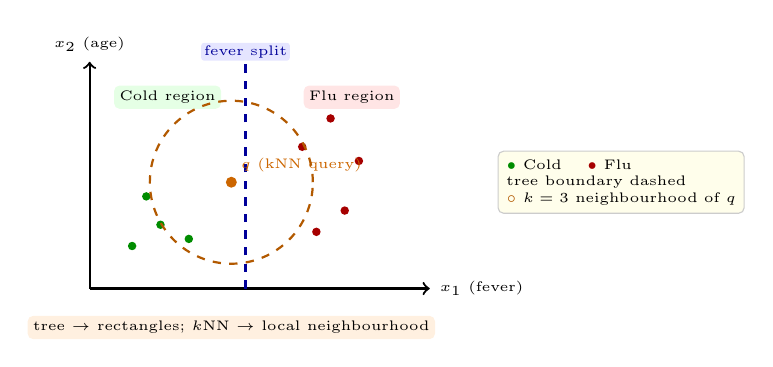
\begin{tikzpicture}[scale=0.9, every node/.style={font=\scriptsize}]
\draw[->, thick] (0,0)--(4.8,0) node[right, font=\tiny] {$x_1$ (fever)};
\draw[->, thick] (0,0)--(0,3.2) node[above, font=\tiny] {$x_2$ (age)};
% points
\foreach \x/\y in {0.6/0.6, 1.0/0.9, 1.4/0.7, 0.8/1.3} \fill[green!55!black] (\x,\y) circle (1.7pt);
\foreach \x/\y in {3.0/2.0, 3.4/2.4, 3.8/1.8, 3.2/0.8, 3.6/1.1} \fill[red!65!black] (\x,\y) circle (1.7pt);
% axis-aligned boundary
\draw[thick, blue!60!black, dashed] (2.2,0)--(2.2,3.2) node[above, font=\tiny, fill=blue!10, rounded corners=1pt, inner sep=1pt] {fever split};
\node[font=\tiny, fill=green!10, rounded corners=2pt, inner sep=2pt] at (1.1,2.7) {Cold region};
\node[font=\tiny, fill=red!10, rounded corners=2pt, inner sep=2pt] at (3.7,2.7) {Flu region};
% query point
\fill[orange!80!black] (2.0,1.5) circle (2.2pt) node[above right, font=\tiny] {$q$ (kNN query)};
% k=3 circle
\draw[thick, orange!70!black, dashed] (2.0,1.5) circle (1.15);
\node[font=\tiny, fill=orange!12, rounded corners=2pt, inner sep=2pt] at (2.0,-0.55) {tree $\to$ rectangles; $k$NN $\to$ local neighbourhood};

\node[font=\tiny, align=left, fill=yellow!8, draw=gray!40, rounded corners=2pt, inner sep=3pt] at (7.5,1.5) {\textcolor{green!55!black}{$\bullet$} Cold \quad \textcolor{red!65!black}{$\bullet$} Flu \\ tree boundary dashed \\ \textcolor{orange!70!black}{$\circ$} $k=3$ neighbourhood of $q$};
\end{tikzpicture}
\caption{Left: geometric view. Decision trees produce axis-aligned regions; $k$NN classifies $q$ by its nearest neighbours (here 2 Cold, 1 Flu $\to$ Cold for $k=3$).}
\label{fig:tree-knn-geometry}
\end{figure}

% ============================================================
\section{Naive Bayes}
\label{sec:naive-bayes}
\paragraph{Intuition.} If we know how often flu causes fever and how common flu is, we can flip the reasoning: given fever, which disease is most likely? Bayes rule does the flip; ``naive'' assumes symptoms are independent given the disease --- often wrong but surprisingly effective.

\paragraph{Derivation.} Posterior for class $c$ given $\mathbf{x}=(x_1,\dots,x_d)$:
\begin{equation}
P(c\mid \mathbf{x}) = \frac{P(c)\,P(\mathbf{x}\mid c)}{P(\mathbf{x})}
\propto P(c)\prod_{j=1}^d P(x_j\mid c)\quad\text{(conditional independence)}.
\end{equation}
Classify as $\hat{y}=\arg\max_c P(c)\prod_j P(x_j\mid c)$ (log-space to avoid underflow: $\sum_j\log P(x_j\mid c)$). For continuous $x_j$, use Gaussian $P(x_j\mid c)=\mathcal{N}(x_j;\mu_{cj},\sigma_{cj}^2)$. Estimate $P(c)$ by frequencies, $P(x_j\mid c)$ by counts (with Laplace smoothing $+\alpha$ to handle unseen combinations).

\begin{lstlisting}[language=Python, caption={Three classifiers side-by-side on a toy 2-D problem.}, label={lst:classifiers}]
import numpy as np
from sklearn.tree import DecisionTreeClassifier
from sklearn.naive_bayes import GaussianNB
from sklearn.neighbors import KNeighborsClassifier

X = np.array([[0,0],[1,0],[0,1],[5,5],[6,5],[5,6]])
y = np.array([0,0,0,1,1,1])  # 0=Cold, 1=Flu

tree = DecisionTreeClassifier(criterion="entropy", max_depth=3, random_state=0)
nb   = GaussianNB()
knn  = KNeighborsClassifier(n_neighbors=3, weights="uniform")

for name, clf in [("Tree",tree),("NB",nb),("3-NN",knn)]:
    clf.fit(X, y)
    print(name, clf.predict([[2,2],[5,4]]))  # expect [0,1] if separable
\end{lstlisting}

% ============================================================
\section{Nearest Neighbours and Evaluation Basics}
\label{sec:knn-eval}
\paragraph{$k$NN.} Memorise all training points. For query $\mathbf{q}$, find $k$ nearest under metric $d$ (Euclidean $d_2$, Manhattan $d_1$, or cosine for text) and vote. $k=1$ has low bias, high variance; larger $k$ smooths the boundary. Needs feature scaling (Ch.~2) and suffers \emph{curse of dimensionality}: in high $d$, all distances look alike, so use PCA or feature selection first. No training time, $O(nd)$ per query --- accelerate with KD-trees or LSH.

\paragraph{Confusion-based metrics.} From counts TP, TN, FP, FN:
\begin{equation}
\text{Acc}=\frac{TP+TN}{N},\ 
\text{Prec}=\frac{TP}{TP+FP},\ 
\text{Rec}=\frac{TP}{TP+FN},\ 
F_1=2\frac{\text{Prec}\cdot\text{Rec}}{\text{Prec}+\text{Rec}}.
\end{equation}
Accuracy misleads on imbalanced data (99\% negatives $\to$ always-negative gets 99\% accuracy but zero recall). Prefer $F_1$ or balanced accuracy; full ROC analysis in Ch.~7.

\begin{lstlisting}[language=Python, caption={Confusion matrix and the accuracy trap on imbalanced data.}, label={lst:metrics}]
from sklearn.metrics import confusion_matrix, classification_report
y_true = [1]*10 + [0]*90    # 10% positive, 90% negative
y_pred_lazy = [0]*100       # ``always negative'' model
print(confusion_matrix(y_true, y_pred_lazy))
print(classification_report(y_true, y_pred_lazy, digits=2))
# Accuracy 0.90 but recall for class 1 = 0.00 -> F1 = 0.00 !
\end{lstlisting}

% ============================================================
% ============================================================
\section{A Comparative View and Practical Tips}
\label{sec:compare-classifiers}
\paragraph{When to prefer which.} Trees excel when interpretability matters and data have mixed types and missing values; they need no scaling but overfit without pruning. Naive Bayes shines for high-dimensional sparse data (text) and tiny training sets; it is fast and calibrated when independence roughly holds. $k$NN has no training but expensive query, needs scaling and is sensitive to irrelevant features.

\begin{center}\small
\begin{tabular}{lccc}
\toprule
 & Trees & Naive Bayes & $k$NN \\
\midrule
Handles mixed types & yes & via discretisation & no (numeric) \\
Needs scaling & no & no & yes \\
Training cost & $O(nd\log n)$ & $O(nd)$ & $O(1)$ \\
Query cost & $O(\text{depth})$ & $O(Cd)$ & $O(nd)$ \\
Interpretability & high & moderate & low \\
\bottomrule
\end{tabular}
\end{center}

\paragraph{Regularisation knobs.} Trees: max depth, min samples per leaf, pruning $\alpha$. Naive Bayes: smoothing $\alpha$, feature selection. $k$NN: $k$, distance, weighting (uniform vs.\ distance-weighted), dimensionality reduction. Always tune via CV, never on test (see Ch.~7).

\paragraph{Common pitfall.} Evaluating on training accuracy. A grown tree can memorise noise. Report stratified CV and inspect confusion, not just a single number.

% ============================================================
% ============================================================
\section{Working Through Entropy by Hand}
\label{sec:entropy-hand}
\paragraph{Example.} At node $S$ with $6$ positives, $4$ negatives: $p_+=0.6$, $p_-=0.4$, so $H(S)=-0.6\log_2 0.6 -0.4\log_2 0.4\approx0.971$ bits. Split on fever $>38$ gives left $(5,1)$ with $H_L\approx0.65$, right $(1,3)$ with $H_R\approx0.81$, weighted $H_{\text{after}}=0.6\cdot0.65+0.4\cdot0.81\approx0.714$, Gain $=0.971-0.714=0.257$ bits.

\paragraph{Gini alternative.} Gini for $S$ is $1-0.6^2-0.4^2=0.48$; after split $G_{\text{after}}=0.6\cdot0.28+0.4\cdot0.375=0.318$, reduction $0.162$. Both criteria agree here; they can differ when splits are unbalanced --- GainRatio corrects Gini's bias toward many-valued splits.

\paragraph{Pruning intuition.} A deep tree fits training quirks; validation error first falls then rises. Cost-complexity finds the sweet spot without a separate validation set for every depth.

% ============================================================
% ============================================================
\section{Worked Example: Tuning a Tree on Churn}
\label{sec:worked-tree}
\paragraph{Data.} Tenure, MonthlyCharges, Contract, SupportCalls $\to$ Churn $\{0,1\}$. A tree with max depth $2$ reaches 78\% CV accuracy; depth $6$ reaches 84\% train but 76\% CV --- overfitting.

\paragraph{Pruning path.} Cost-complexity sequence for $\alpha=0,0.005,0.01,0.02$ gives nodes $31,18,9,5$ and CV AUC $0.82,0.84,0.83,0.79$. The best $\alpha=0.005$ balances fit and generalisation.

\paragraph{Comparison.} Naive Bayes on the same data (with discretised charges) scores 80\% CV but calibrates well for ranking. $k$NN with $k=7$ after standardisation scores 79\% but is slower at prediction time. The tree wins on interpretability for business stakeholders.

\begin{lstlisting}[language=Python, caption={Cost-complexity pruning path for decision trees.}, label={lst:prune}]
from sklearn.tree import DecisionTreeClassifier
from sklearn.model_selection import cross_val_score
import numpy as np
X, y = np.random.randn(400,4), np.random.randint(0,2,400)
path = DecisionTreeClassifier(random_state=0).cost_complexity_pruning_path(X,y)
for ccp in path.ccp_alphas[::4]:
    clf = DecisionTreeClassifier(ccp_alpha=ccp, random_state=0)
    print(f"ccp={ccp:.4f}  CV={cross_val_score(clf,X,y,cv=3).mean():.3f}")
\end{lstlisting}
\paragraph{Reading the pruning path.} The sequence of alpha values tells a story of complexity traded for stability across folds.
At alpha zero the tree memorises rare contract combinations that will not recur next quarter.
At alpha 0.005 the tree keeps the splits on tenure and contract that replicate across folds.
Beyond that the tree becomes a stump that underfits, missing the interaction between support calls and monthly charges.
\paragraph{Practical model choice.} The two-point gap between the tree and Naive Bayes matters less than who must act on the prediction.
Retention teams prefer the tree because each path reads as a rule they can attach an offer to.
Naive Bayes earns its place when calibrated churn probabilities feed a budget allocator rather than a call list.
The kNN result warns that standardisation and serving latency must be weighed alongside raw accuracy.
\paragraph{Lessons for larger data.} On millions of rows the pruning path is computed on a stratified sample first, then confirmed at scale.
Categorical cardinality explodes tree depth, so high-cardinality fields are grouped before splitting.
Missing contract values are routed with surrogate splits rather than dropped, preserving the deployment population.
\paragraph{Takeaway for deployment.} Freeze the chosen alpha, retrain on all labelled data, and log the tree rules alongside the code version.
Monitor leaf-level churn rates monthly, since a leaf that decays signals concept drift before global accuracy moves.
Re-tune only when the monitored gap exceeds the cross-validation standard error observed during selection.
That discipline turns a classroom pruning exercise into a maintainable retention model.
Students should rerun the listing with different seeds to feel how stable the chosen alpha really is.

% ============================================================
\section{Support Vector Machines and the Kernel Trick}
\label{sec:svm}
\paragraph{Margin intuition.} Among all boundaries separating two classes, the SVM picks the one with the widest safety corridor: points closest to the boundary (the \emph{support vectors}) alone determine it, so moving any other point changes nothing. Formally it minimises $\frac{1}{2}\lVert\mathbf{w}\rVert^2$ subject to $y_i(\mathbf{w}^\top\mathbf{x}_i+b)\geq 1$, giving margin width $2/\lVert\mathbf{w}\rVert$. A soft margin adds slack $\xi_i\geq 0$ with penalty $C\sum_i\xi_i$, letting a few outliers cross at a price: large $C$ punishes violations harshly (narrow, fussy margin), small $C$ tolerates them (wide, forgiving margin).
\paragraph{Kernel trick.} Rings or XOR patterns are not linearly separable, so map $\mathbf{x}\mapsto\phi(\mathbf{x})$ into a higher-dimensional space where they are --- but never compute $\phi$ explicitly, since training only needs inner products $K(\mathbf{x},\mathbf{z})=\phi(\mathbf{x})^\top\phi(\mathbf{z})$ (RBF $K=\exp(-\gamma\lVert\mathbf{x}-\mathbf{z}\rVert^2)$, polynomial $(1+\mathbf{x}^\top\mathbf{z})^p$). The kernel is thus a similarity dial: RBF declares far-apart points dissimilar, and $\gamma$ sets how fast similarity decays.
\paragraph{Worked 2D example.} Positives $(2,2),(2,3)$, negatives $(0,0),(1,0)$: the boundary $x_2=1$ with $\mathbf{w}=(0,1)$, $b=-1$ satisfies $y_i(\mathbf{w}^\top\mathbf{x}_i+b)\geq 1$ with equality on $(2,2)$, $(0,0)$, $(1,0)$ --- three support vectors --- and margin width $2/\lVert\mathbf{w}\rVert=2$. No other point matters: deleting $(2,3)$ leaves the boundary unchanged, which is exactly why max-margin generalises.
% ============================================================
\section{From Labels to Numbers: Regression and Regularisation}
\label{sec:regression}
\paragraph{Intuition.} Regression predicts a number (price, temperature) instead of a label but reuses the same linear score $f(\mathbf{x})=\mathbf{w}^\top\mathbf{x}+b$: classification thresholds it, regression reports it. Least squares minimises $\sum_i(y_i-f(\mathbf{x}_i))^2$ with closed form $\hat{\mathbf{w}}=(X^\top X)^{-1}X^\top\mathbf{y}$.
\paragraph{Regularisation intuition.} With many features, least squares memorises noise via huge cancelling weights. Ridge adds $\lambda\lVert\mathbf{w}\rVert_2^2$ (shrinks every weight smoothly); LASSO adds $\lambda\lVert\mathbf{w}\rVert_1$ (drives some weights exactly to zero, hence selects features). Larger $\lambda$ means a simpler, stabler fit; tune it by cross-validation (Ch.~7), exactly like tree depth or $k$.
\paragraph{Worked fit.} Points $(0,1),(1,3),(2,7)$: least squares gives $y=3x+2/3$ (slope $3$, intercept $0.67$) with residuals $1/3,-2/3,1/3$. Centred ridge with $\lambda=1$ pulls the slope to $6/(2+1)=2$, trading a little training error for stability --- the same bias-variance trade-off behind pruning and large $k$.
\paragraph{Practical pick.} Few thousand dense points: standardise, then try RBF-SVM against logistic regression. Sparse 10k-feature text: prefer a linear SVM (fast, strong baseline). More features than rows: reach for LASSO first, since it discards irrelevant features for you.
\paragraph{Common pitfall.} Tuning $C$, $\gamma$, or $\lambda$ on the test set fakes the score; tune on validation folds and report test once --- Ch.~7's discipline applies to every knob in this chapter.
\begin{lstlisting}[language=Python, caption={SVM with RBF kernel beside regularised regression.}, label={lst:svm-reg}]
from sklearn.svm import SVC
from sklearn.linear_model import Ridge, Lasso
SVC(C=1.0, kernel="rbf", gamma="scale").fit(X, y)  # max margin + kernel trick
Ridge(alpha=1.0).fit(Xr, yr)  # L2 shrinkage; Lasso(alpha=0.1) sparsifies
\end{lstlisting}
% ============================================================
\section{Chapter Notes}
Decision trees: Quinlan ID3/C4.5, Breiman CART. Naive Bayes despite independence often rivals more complex models on text. $k$NN is a lazy learner --- analysis via Cover-Hart (1967): asymptotically error $\le 2\times$ Bayes optimal. For imbalance and ROC beyond accuracy, see Ch.~7.

% ============================================================
\section{Exercises}
\begin{enumerate}[label=E3.\arabic*, leftmargin=*, itemsep=0.6em]
    \item \textbf{Entropy split.} A node has $6$ Flu, $4$ Cold. Split A gives children $(4,1)$ and $(2,3)$; split B gives $(3,2)$ and $(3,2)$. Compute $H$ and Gain for each and choose the better split.
    \item \textbf{Naive Bayes by hand.} Classes $C\in\{S,H\}$ with $P(S)=0.7$. Likelihoods $P(\text{fever}\mid S)=0.1$, $P(\text{fever}\mid H)=0.6$. Observe fever. Compute $P(S\mid\text{fever})$ and $P(H\mid\text{fever})$, and classify with and without Laplace smoothing if one count was zero.
    \item \textbf{$k$NN geometry.} Points $(0,0):0,(1,0):0,(0,1):0,(3,3):1$. Query $(1,1)$. Classify for $k=1,3,4$ with Euclidean distance. Explain how increasing $k$ changes bias and variance.
    \item \textbf{Metrics.} Given $TP=30,FP=10,FN=20,TN=40$, compute accuracy, precision, recall, $F_1$. Construct a case where accuracy $=95\%$ but recall $<10\%$, and explain why $F_1$ is preferred.
    \item \textbf{Overfitting trees.} Explain why an unpruned tree achieves $100\%$ training accuracy yet may generalise poorly. Propose two pruning heuristics and sketch how $\alpha$ in $R_\alpha(T)$ controls complexity.
\end{enumerate}
% End of Chapter 3
